\begin{frame}
    % The problem we are faced with is referred to as \textbf{Temporal Action Segmentation} or \textbf{Video Classification}.

    \centering
    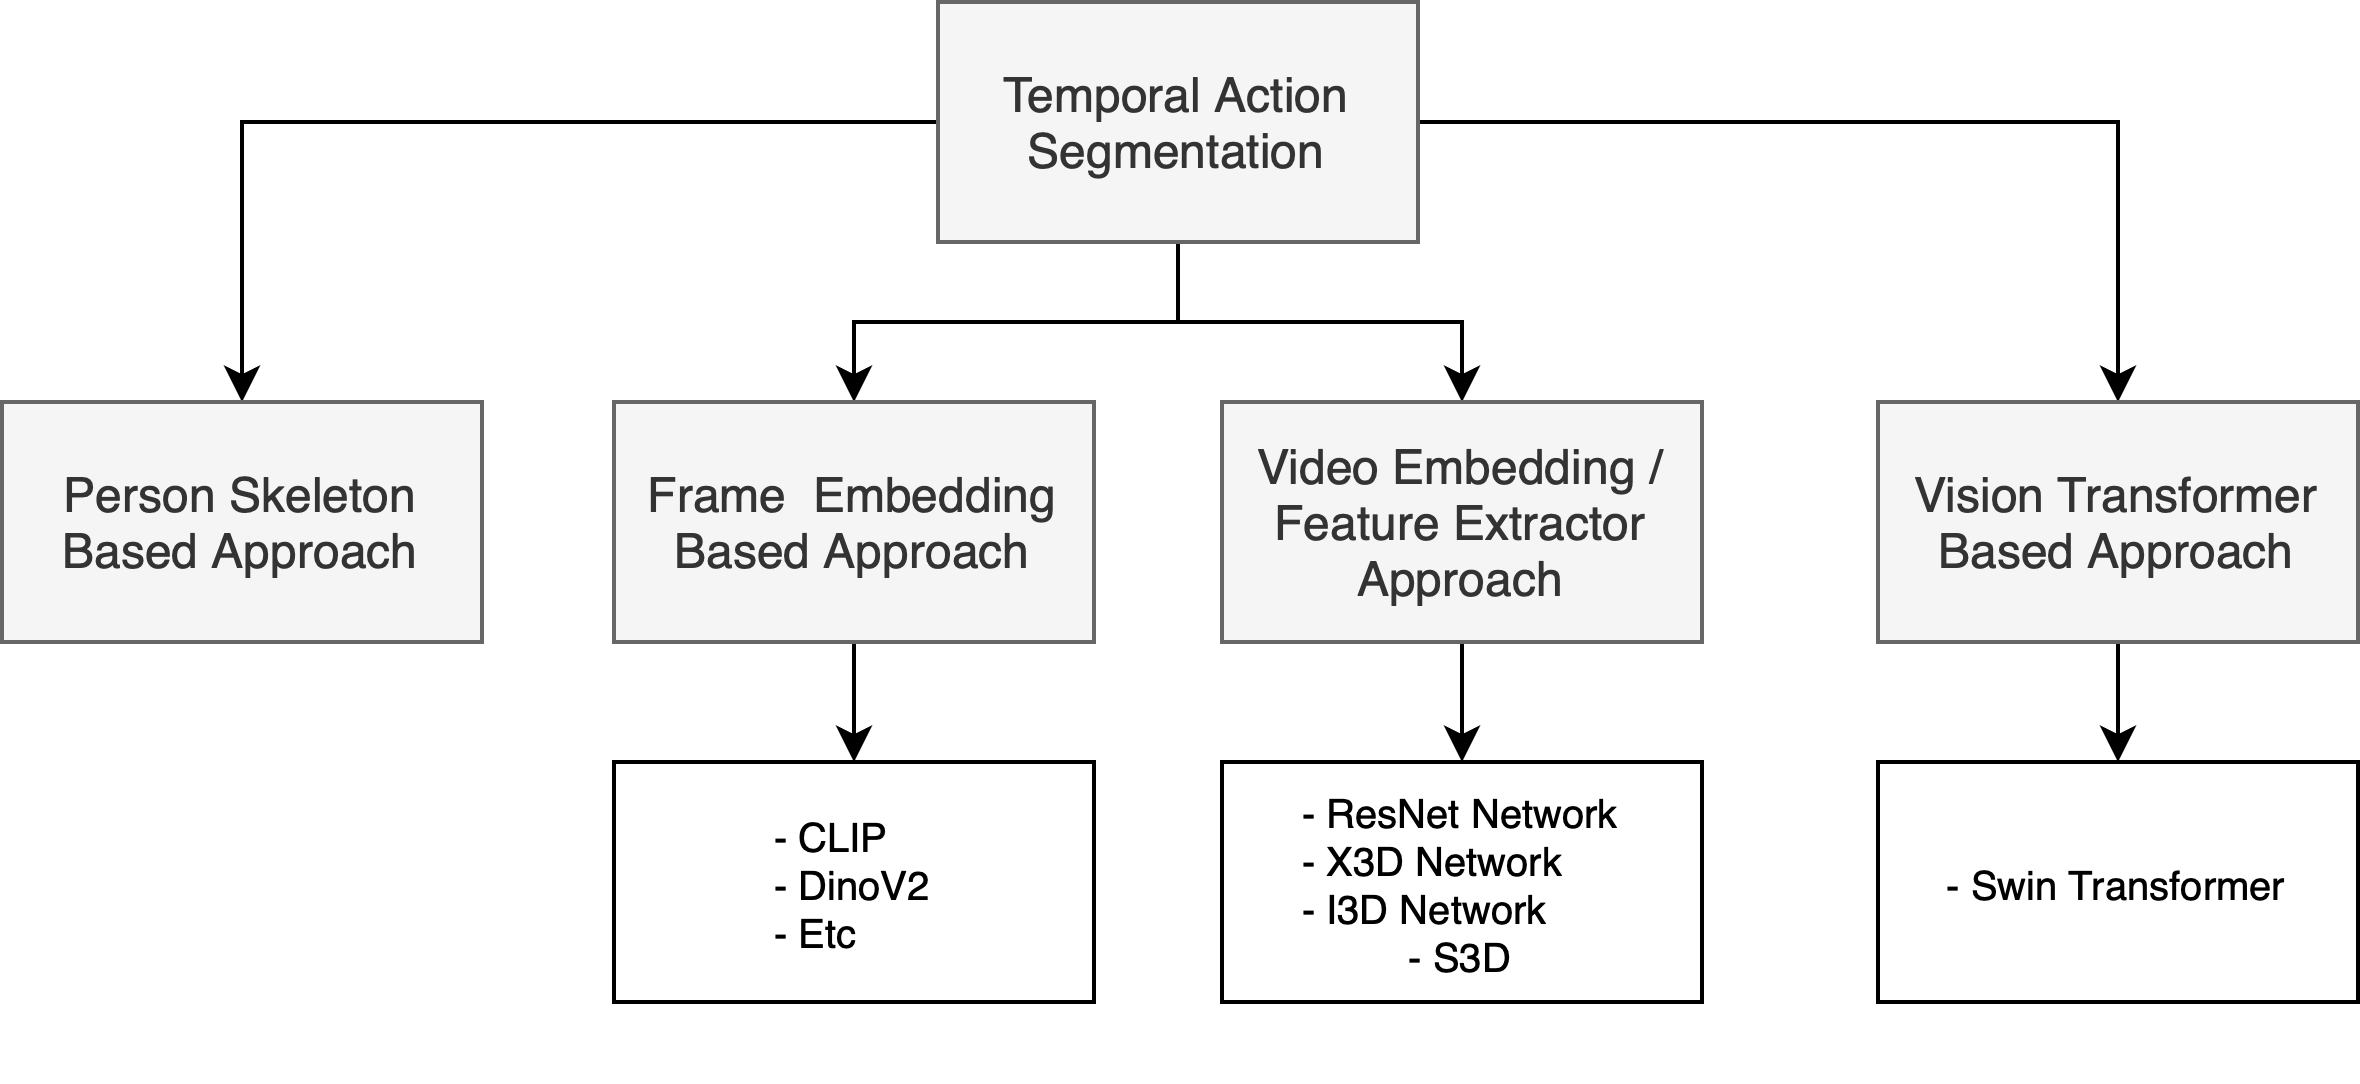
\includegraphics[width=0.75\textwidth]{assets/visuals/usual-solutions-visual.drawio.png}
\end{frame}

% NOTE: say what the embedding models tries to do.

% NOTE: talk about semi supervised learning methods or unsupervised learning methods.
% NOTE: explain quickly the neural networks cited above.
% NOTE: for 3D CNNs to perform classification on small portions of the videos (usually from 8 to 32 frames).

% NOTE: about skeleton based approach: When Humans are involved some techniques (Cite the papers that uses this techniques) uses the humans skeletons points to perform classification.

% TODO: cite other models from the SOTA recap paper
% TODO: cite all the models
% TODO: cite at least a paper that uses a skeleton based approach.

% S3D: https://arxiv.org/pdf/1807.08069
% SlowFast: 
% ResNet:
% X3D: 
% I3D: (https://github.com/piergiaj/pytorch-i3d)
% Swin Transformer: https://arxiv.org/pdf/2106.13230